\chapter{Introduction}


\chapter{NDP architecture}
NDP is a network architecture for datacenters with Clos topology. 
The primary goals are low completion latency for short flows and predictable high throughput for longer flows.

The architecture includes switches and endpoints...


\section{Clos topology}
Clos network...
Spine and leaf nodes/switches
% describe more universally networks with more levels?
every leaf connected to every spine node
easily scalable for higher bandwidth and reliability by adding more spine and leaf nodes
low cost (expand why)
dual attach - machine is connected to two leaf switches for redundancy
spine nodes are connected to exit leaves

The topology is designed to allow communication of every node with another at full connection speed.
This requires splitting the sent data on different paths to ensure even flow of data and to evade congestion where more paths of different flows could meet.
This requires a lot of reordering at the endpoints and thus large buffers for the received data.


\section{Precedent solutions}
It was created to provide better latency than existing protocols for congestion control like Data Center TCP or Cut Payload.

Newer solution is RDMA over Converged Ethernet v2 using Ethernet flow control in switches. It provides good latency for datacenter workloads until loaded more heavily.
When loaded, packets build up in switch queues. The switches then generate PFC pause frames, which negatively impact the network latency.

Applications try to reuse TCP connections to lower the cost of TCP handshake.


\section{Datacenter}
Usual applications are computations using RPC or similar protocol. The average utilization of network is not extremly high, but the load comes often in bursts.

Computation in datacenters usually require sending task from one node to other workers and then recieving the results back to single node. This traffic causes problem named incast.


\section{Design}
The reference implementation from original paper uses DPDK on Linux for end-host.
The part for switches was implemented as software switch, for NetFPGA hardware switch and in P4.

Congestion control - one receiver from many senders.
Spread the flow to multiple paths - huge reordering.

Inspired by Cut Payload design.
Two priority queues for data packets and returning headers in ratio 1:10.
NACK header returns instantly to notify the sender.

Phase effect.



\chapter{XDP}
% reader should know about the linux kernel, but not in this depth

\section{Original/classic BPF}
Berkeley Packet Filter
used by tcpdump for filtering
today obsolete, referred as classic bpf, because eBPF is often reffered as BPF
today's kernel translates it to ebpf
% https://docs.cilium.io/en/v1.8/bpf/


\section{eBPF}
extended Berkeley Packet Filter
When running in user-space, packets must be copied across the kernel/user-space protection boundary
history of creation of bpf

roots in software-defined networking (SDN)
iptables created in 1999
iptables didn't scale for the evolving containerization (Kubernetes)
In 2014 when Kubernetes started, the first eBPF patch was also merged to the Linux kernel.
In 2015 the eBPF backend was merged to the LLVM compiler suite so the compiler was able to produce eBPF bytecode.
The eBPF was also integrated to the Linux kernel's traffic control, which made the networking programmable using the eBPF language.
% https://cilium.io/blog/2020/11/10/ebpf-future-of-networking/

Can store data in maps/hashes


\section{XDP}
Stands for eXpress Data Path 
started in 2016 (first merge in Linux kernel)
Packet processor in the Linux networking data path
Focused on performance
Uses eBPF language for packet processing.
Runs in kernel.
Subset of C.
Must terminate, no locking
Not a kernel bypass
XDP has got write access to raw packet
Recycles pages to lower the usage of malloc/free.

Though still in developmnet during writing this thesis, it is already used in production for packet filtering and processing by large companies like Facebook
\footnote{http://vger.kernel.org/lpc-networking2018.html\#session-10}
\footnote{http://vger.kernel.org/lpc-networking2018.html\#session-15}.

Can be used for filtering DOS attacks before processing the packet in network stack, Layer-4 load balancing, forwarding, flow sampling and monitoring.
Add or pop encapsulation headers, modify packet header before forwarding.
Possible function as a software router depend on multi-port TX (probably not implemented yet).
Bridge to virtual machines.

Can be offloaded to network card/NIC that supports the BPF code.
The XDP program can be loaded in several modes\footnote{https://pantheon.tech/what-is-af\_xdp/}:
\begin{itemize}
    \item \emph{Generic} when the NIC driver doesn't support the XDP framework.
        The kernel simulates the work of the driver, but doesn't bring any perceptible performance boost, because the packets are still always loaded to the kernel stack to be processed.
        This is usually the case of generic network drivers in home computers, laptops and virtualized hardware.
    \item \emph{Native} when the code is passed to the NIC driver, which executes the actions without interaction of the kernel.
        There is still a short list of drivers supporting the XDP and they are mostly from the enterprise segment.
    \item \emph{Offloaded} when the NIC supports direct execution in its hardware. This allows the processing of packets outside of CPU and spares the computation power for more important tasks. Few NICs currently support this.
\end{itemize}

The offloading can allow for example decentralized NIC switching\footnote{https://ieeexplore.ieee.org/document/6866848} without the interference of the CPU.

Returns action: pass, drop, forward (TX), or abort meaning fail in the eBPF program.

XDP also provides new socket \texttt{AF\_XDP}, which is available from kernel version 4.18.
It does not completly bypass the kernel stack, but works similarly to \texttt{AF\_PACKET} or DPDK.


\subsection{Comparison with DPDK}
XDP is meant as OSS alternative to DPDK.

It is a new layer in the Linux kernel network stack.
It runs in kernel space, which offers reusage of mechanisms already implemented in kernel.
DPDK runs in user space, entirely skipping the kernel and thus the user needs to implement everyting there.

It takes action before allocation of socket buffer, which allows much faster action with the packet, before the packet continues further through the network stack.

The DPDK usually needs a dedicated CPU to work on, while the XDP doesn't need a full separate CPU core.

The performance of the XDP is in genral still behind the DPDK, despite continuously catching up.
\footnote{http://vger.kernel.org/lpc\_net2018\_talks/presentation-lpc2018-xdp-future.pdf}
Still offers huge performance gain compared to iptables without using the XDP.
\ref{fig:drop-test}

\begin{figure}
  \centering
  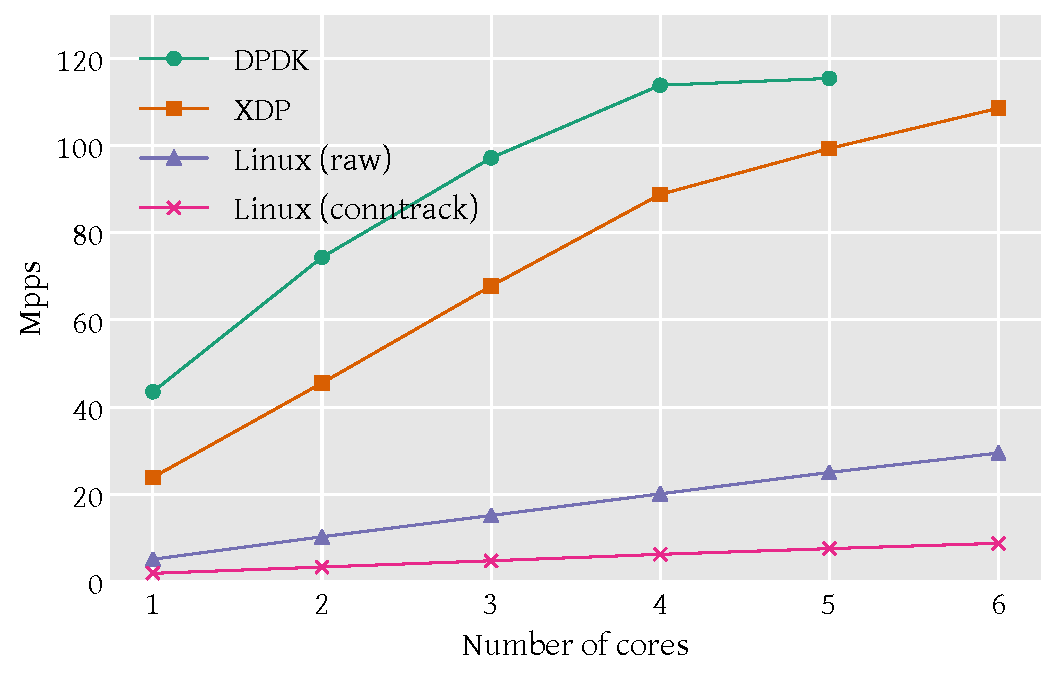
\includegraphics[width=12cm]{drop-test}
  \caption{Performance of XDP compared to DPDK and Linux without XDP on packet dropping measured in millions of packets per second. Measurement if from the end of the year 2018. (https://github.com/tohojo/xdp-paper)}
  \label{fig:drop-test}
\end{figure}

\chapter{Implementation}

\chapter{Evaluation}
